\documentclass{report}

\input{preamble}
\input{macros}
\input{letterfonts}

\title{\Huge{Math 120 QR}}
\author{\huge{Alex Hernandez Juarez}}
\date{Fall 2024}

\begin{document}

\maketitle
\newpage% or \cleardoublepage
% \pdfbookmark[<level>]{<title>}{<dest>}
\pdfbookmark[section]{\contentsname}{toc}
\tableofcontents
\pagebreak

\chapter{}
\section{PSet 1}

\qs{}{Find the lengths of the sides of the triangle with vertices P (2, 1, 3), Q(0, 2, 5) and R(4, -1, 4). Is the
triangle an acute triangle (all sides less than 90$^{\circ}$), a right triangle, or an obtuse triangle (one angle
greater than 90$^{\circ}$)}

\sol{
	Image: 
	\tdplotsetmaincoords{60}{120}
	\begin{tikzpicture}[tdplot_main_coords, scale=1]

		% Define the coordinates
		\coordinate (P) at (2, 1, 3);
		\coordinate (Q) at (0, 2, 5);
		\coordinate (R) at (4, -1, 4);
		
		% Draw the axes
		\draw[thick, -stealth] (0,0,0) -- (5,0,0) node[anchor=north east]{$x$};
		\draw[thick, -stealth] (0,0,0) -- (0,5,0) node[anchor=north west]{$y$};
		\draw[thick, -stealth] (0,0,0) -- (0,0,5) node[anchor=south]{$z$};
		
		% Draw the triangle
		\draw[thick] (P) -- (Q) -- (R) -- cycle;
		
		% Label the points
		\node at (2, 1, 3) [anchor=south west] {P(2, 1, 3)};
		\node at (0, 2, 5) [anchor=south east] {Q(0, 2, 5)};
		\node at (4, -1, 4) [anchor=north west] {R(4, -1, 4)};
		
	\end{tikzpicture}
	
	\begin{center}
		\[ \ray{PQ} = \langle 0 - 2, 2 - 1, 5 - 3 \rangle = \langle -2, 1, 2 \rangle \]
		\[ \ray{QR} = \langle 4 - 0, -1 - 2, 4 - 5 \rangle = \langle 4, -3, -1 \rangle \]
		\[ \ray{RP} = \langle 2 - 4, 1 - -1, 3 - 4 \rangle = \langle -2, -2, 1 \rangle \]
		\[ |\ray{PQ}| = \sqrt{(-2)^{2} + {1}^{2} + (-2)^{2}} = \sqrt{9} = 3\]
		\[ |\ray{QR}| = \sqrt{(4)^{2} + (-3)^{2} + (1)^{2}} = \sqrt{26}\] 
		\[ |\ray{RP}| = \sqrt{(-2)^{2} + (-2)^{2} + (1)^{2}} = \sqrt{9} = 3 \] 
	\end{center}
	angles: 
	\begin{center}
		\[ |\ray{PQ}|^{2} = 26 = 9 + 9 - 2(3)(3) \cos{\theta}\]
		\[ 8 = - 18 \cos{\theta}\]  
		\[ \frac{8}{18} = - \cos(\theta)\]
		\[ \theta = \arccos\left(-\frac{8}{18}\right) \approx 116\]  
	\end{center}
	Trianlge is obtuse 
}



\qs{}{Find the equation of the sphere for which the line segment between the points 
	$A(1,1,1)$ and $B(3,-7,-3)$ is a diameter. (This means that that $A$ and $B$ are antipodal points on the sphere.)
}

\sol{
	\\
	Center of sphere: 
		\begin{center}
			\[ \frac{x_{1} + x_{2}}{2}, \frac{y_{1} + y_{2}}{2},  \frac{z_{1} + z_{2}}{2}  = \frac{1 + 3}{2},  \frac{1 + -7}{2}, \frac{1 +  - 3}{2} = (2, -3, -1) \] 
		\end{center}
	Dimaeter: 
		\begin{center}
			\[ \sqrt{(3-1)^{2} + (-7 - 1)^{2} + (-3-1)^{2}} =  4\sqrt{6} \] 
		\end{center}
	Radius: 
		\begin{center}
			\[ r = \frac{4\sqrt{6}}{2} = 2\sqrt{6}\] 
		\end{center}
	Equation of sphere: 
		\begin{center}
			\[ (x-2)^{2} + (y+3)^{2} + (z-2)^{2} = (3\sqrt{2})^{2}\] 
			\[ (x-2)^{2} + (y+3)^{2} + (z-2)^{2} = 18 \] 
		\end{center}
}

\newpage

\qs{}{
	a) Describe in words and with a sketch the regions in $\mathbb{R}^{3}$ represented by \\
		i. The equation $z = -2$ \\
		ii. The inequality $x^{2} + (y-1)^{2} + (z+1)^{2}  \leq 9$   \\
	b) In your sketch, shade in the intersection of the two regions you drew in part (a), i.e., the set of
	all points $(x,y,z)$ in $\mathbb{R}^{3}$ satisfying both $ z= - 2$ and $x^{2} + (y - 1)^{2} + (z+1)^{2} \leq 9 $ 
}

\sol{
	\\
	a) \\
	i. Represents a plane in $\mathbb{R}^{3}$ that is parallel to the $xy$-plane and liest at a height of -2 units below the $xy$-plane. This plane contains all points 
	where the $z$-cooridnate is -2, regardless of the $x$ and $y$ values. 
	\begin{center}
		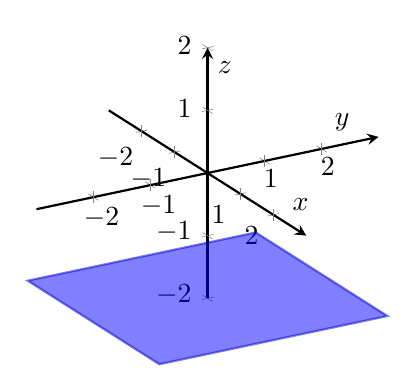
\begin{tikzpicture}
			\begin{axis}[
				axis lines=middle,
				xlabel={$x$},
				ylabel={$y$},
				zlabel={$z$},
				xmin=-3, xmax=3,
				ymin=-3, ymax=3,
				zmin=-2, zmax=2,
				xtick={-2,-1,0,1,2},
				ytick={-2,-1,0,1,2},
				ztick={-2,-1,0,1,2},
				enlargelimits=false,
				view={60}{30},
				grid=major,
				thick,
			]
			% Drawing the plane z = -2
			\addplot3[surf, domain=-2:2, domain y=-2:2, samples=2, opacity=0.5] 
			{ -2 };
			\end{axis}
		\end{tikzpicture} 
	\end{center}
	ii. A solid sphere in $\mathbb{R}^{3}$  with the center at point (0,1,-1) and a radius of 3. This indluces all the points inside and on the surface 
	of the sphere.
	\begin{center}
		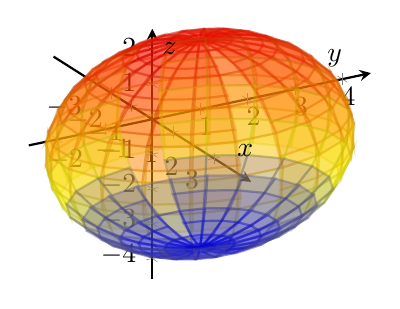
\begin{tikzpicture}
			\begin{axis}[
				axis lines=middle,
				xlabel={$x$},
				ylabel={$y$},
				zlabel={$z$},
				xmin=-4, xmax=4,
				ymin=-2, ymax=4,
				zmin=-4, zmax=2,
				xtick={-3,-2,-1,0,1,2,3},
				ytick={-2,-1,0,1,2,3,4},
				ztick={-4,-3,-2,-1,0,1,2},
				enlargelimits=true,
				view={60}{30},
				grid=major,
				thick,
				samples=20,
			]
			% Drawing the sphere x^2 + (y - 1)^2 + (z + 1)^2 <= 9
			\addplot3[surf, opacity=0.3, domain=-3:3, y domain=-2:4] 
			({3*cos(deg(x))*sin(deg(y))}, {1+3*sin(deg(x))*sin(deg(y))}, {-1+3*cos(deg(y))});
			\end{axis}
		\end{tikzpicture} 
	\end{center}


	b) 
	\begin{center}
		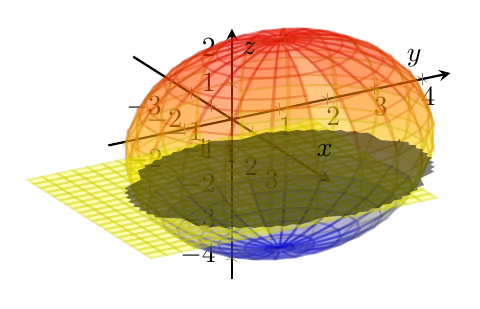
\begin{tikzpicture}
			\begin{axis}[
				axis lines=middle,
				xlabel={$x$},
				ylabel={$y$},
				zlabel={$z$},
				xmin=-4, xmax=4,
				ymin=-2, ymax=4,
				zmin=-4, zmax=2,
				xtick={-3,-2,-1,0,1,2,3},
				ytick={-2,-1,0,1,2,3,4},
				ztick={-4,-3,-2,-1,0,1,2},
				enlargelimits=true,
				view={60}{30},
				grid=major,
				thick,
				samples=20,
			]
			% Drawing the sphere x^2 + (y - 1)^2 + (z + 1)^2 <= 9
			\addplot3[surf, opacity=0.2, domain=-3:3, y domain=-2:4] 
			({3*cos(deg(x))*sin(deg(y))}, {1+3*sin(deg(x))*sin(deg(y))}, {-1+3*cos(deg(y))});
			
			% Drawing the plane z = -2
			\addplot3[surf, opacity=0.3, domain=-3:3, y domain=-3:3] 
			({x}, {y}, {-2});
			
			% Shading the intersection circle
			\addplot3[fill=black, fill opacity=0.5, draw=none, domain=0:360, samples=50] 
			({3*cos(deg(x))}, {1+3*sin(deg(x))}, {-2});
			\end{axis}
		\end{tikzpicture}
	\end{center}
}

\qs{}{Describe in words the region(s)  $\mathbb{R}^{3}$ represented by the inequality $x^{2} \leq 9$  }

\sol{
	It is the set off all points that lite within the planes $x = -3$ and $ x= 3$. It is a 3-dimensional
	slab that extends infinitely in teh $y$ and $z-$ directions, but is bounded by $x = -3$ and $x=3$ along the x-axis. 
}


\newpage 

\qs{}{Let $A, B, C, D$, and $E$ be the points in the diagram below. Write each combintation 
	of vectors as a single vector. \\
	1. $\ray{AE} + \ray{ED}$ \\
	2. $\ray{AC} - \ray{AB}$ \\
	3. $\ray{AC} + \ray{EA}$ \\
	4. $\ray{AC} + \ray{ED} + \ray{DC} + \ray{CB} + \ray{BA}$ 
	\insertpng[.75]{Prob.png}
}

\sol{
	\\
	1. $\ray{AE} + \ray{ED} = \ray{AD}$  \\
	2. $\ray{AC} - \ray{AB} = (\ray{AC} + \ray{BC}) - \ray{AB} = \ray{BC}$ \\
	3. $\ray{AC} + \ray{EA} = \ray{AC} - \ray{AE} = \ray{EC} $ \\
	4. $\ray{AC} + \ray{ED} + \ray{DC} + \ray{CB} + \ray{BA}:  $ 
		\begin{center}
			\[ \ray{ED} + \ray{DC} = \ray{EC} \]
			\[ \ray{CB} + \ray{BA} = \ray{CA}\] 
			\[ \ray{AC} + \ray{EC} + \ray{CA} = \ray{EA}\]   
		\end{center}
}

\newpage 


\qs{}{Find the sum of the vectors $\vec{a} = \langle 2, -3 \rangle$ and $\vec{b} = \langle 1, 4 \rangle$ and illustrate geometrically}

\sol{
	\begin{center}
		\[ \vec{a} + \vec{b}= \langle 2, -3 \rangle + \langle 1, 4 \rangle \] 
		\[ \vec{a} + \vec{b}= \langle 2 + 1, -3 + 4\rangle = \langle 3, 1 \rangle  \] 
	\end{center}
	
	\begin{center}
		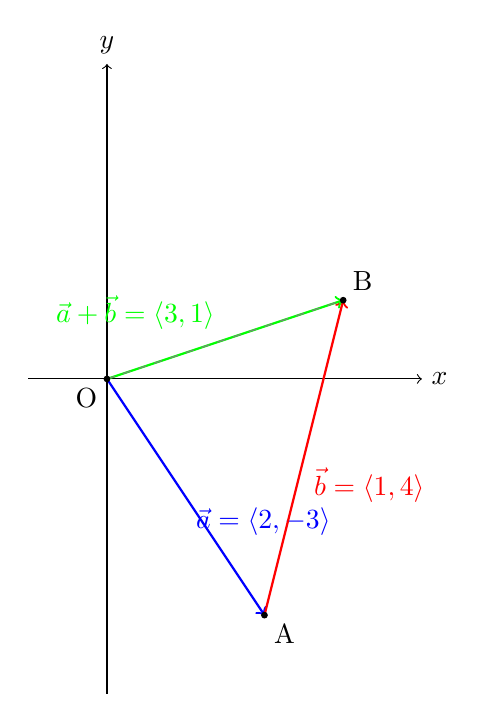
\begin{tikzpicture}
			% Draw the x and y axis
			\draw[->] (-1,0) -- (4,0) node[right] {$x$};
			\draw[->] (0,-4) -- (0,4) node[above] {$y$};
			
			% Draw vector a
			\draw[->, thick, blue] (0,0) -- (2,-3) node[midway, below right] {$\vec{a} = \langle 2, -3 \rangle$};
			
			% Draw vector b from the tip of vector a
			\draw[->, thick, red] (2,-3) -- (3,1) node[midway, below right] {$\vec{b} = \langle 1, 4 \rangle$};
			
			% Draw vector a+b
			\draw[->, thick, green] (0,0) -- (3,1) node[midway, above left] {$\vec{a} + \vec{b} = \langle 3, 1 \rangle$};
			
			% Draw dashed line from origin to b
			\draw[dashed, gray] (0,0) -- (3,1);
			
			% Add points for the vectors
			\filldraw[black] (0,0) circle (1pt) node[below left] {O};
			\filldraw[black] (2,-3) circle (1pt) node[below right] {A};
			\filldraw[black] (3,1) circle (1pt) node[above right] {B};
		\end{tikzpicture}
	\end{center}

}

\qs{}{Find the vector that has the same direction as $\hat{\imath} + 3 \hat{\jmath} - \hat{k}$ but has length 6  }

\sol{
	\begin{center}
		\[ \hat{u} = \frac{\mathbf{v}}{|\mathbf{v|}} = \frac{1}{\sqrt{11}}\hat{\imath} + \frac{3}{\sqrt{11}}\hat{j} - \frac{1}{\sqrt{11}} \hat{k} \] 
		\[ \mathbf{u} \times \hat{u} = 6 \times \left( \frac{1}{\sqrt{11}}\hat{\imath} + \frac{3}{\sqrt{11}}\hat{j} - \frac{1}{\sqrt{11}} \hat{k} \right) \] 
		\[ \mathbf{u} = \frac{6}{\sqrt{11}}\hat{\imath} + \frac{18}{\sqrt{11}}\hat{j} - \frac{6}{\sqrt{11}} \hat{k} \] 
	\end{center}
}

\qs{}{omplete the Ximera assignment on vector projections linked from the Problem Set 1 assignment in
the Canvas umbrella site. Write “I have completed the Ximera assignment” for Problem 8 on the file
you submit for this problem set.}

\sol{“I have completed the Ximera assignment”  }


\end{document}
